\documentclass{article}
\usepackage{tikz}
\usetikzlibrary{arrows}
\begin{document}
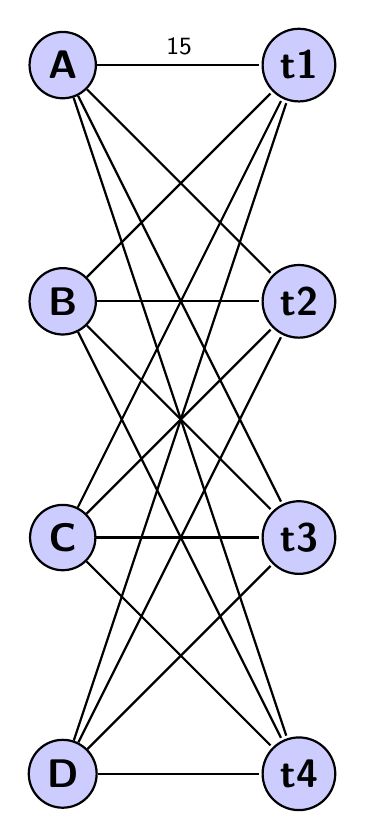
\begin{tikzpicture}[-,>=stealth',shorten >=1pt,auto,node distance=3cm,
  thick,main node/.style={circle,fill=blue!20,draw,font=\sffamily\Large\bfseries}]

  \node[main node] (A) {A};
  \node[main node] (B) [below of=A] {B};
  \node[main node] (C) [below  of=B] {C};
  \node[main node] (D) [below of=C] {D};
  \node[main node] (t1) [right of=A]{t1};
  \node[main node] (t2) [right of=B] {t2};
  \node[main node] (t3) [right of=C] {t3};
  \node[main node] (t4) [right of=D] {t4};

  \path[every node/.style={font=\sffamily\small}]
    (A) edge node[above] {15}  (t1)
        edge  (t2)
        edge  (t3)
        edge  (t4)
    (B) edge  (t1)
        edge  (t2)
        edge  (t3)
        edge  (t4)
    (C) edge  (t1)
        edge  (t2)
        edge  (t3)
        edge  (t4)
    (D) edge  (t1)
        edge  (t2)
        edge  (t3)
        edge  (t4)
        ;
\end{tikzpicture}
\end{document}